\pdfoutput=1
\PassOptionsToPackage{table}{xcolor}

\documentclass[11pt]{article}
\usepackage[final]{acl}


\usepackage{times}
\usepackage{latexsym}
\usepackage{amsmath}
\usepackage{listings}
\usepackage{caption}
\usepackage{subcaption}
\usepackage{chngcntr}
\usepackage[T1]{fontenc}
\usepackage[utf8]{inputenc}
\usepackage{microtype}
\usepackage{multirow}
\usepackage{colortbl}
\usepackage{enumitem}
\usepackage{amssymb}
\usepackage[colaction]{multicol}


\newcommand\multicollinenumbers{
 \linenumbers
 \def\makeLineNumber{\docolaction{\makeLineNumberLeft}{}{\makeLineNumberRight}}}


\newcommand{\checkedbox}{\ensuremath{\rlap{\checkmark}\square}}


\usepackage{placeins}
\usepackage{threeparttable}
\usepackage{inconsolata}
\usepackage{xspace}
\usepackage{pdfpages}
\usepackage{graphicx}
\lstset{breaklines=true}
\usepackage{paracol}
\usepackage{tgtermes}
\usepackage{xspace}

\newcommand{\sysname}{{\textit{\textmd{\fontfamily{qtm}\selectfont MIBot}}}\xspace}

\newcommand{\sysnamewithv}{{\textit{\textmd{\fontfamily{qtm}\selectfont MIBot v6.3A}}}\xspace}

\newcommand{\oldsysname}{{\textit{\textmd{\fontfamily{qtm}\selectfont MIBot v5.2}}}\xspace}

\usepackage{titlesec}
\usepackage[most]{tcolorbox}
\usepackage{array}
\usepackage{tabularx}
\definecolor{darkblue}{rgb}{0.1, 0.2, 0.6}
\definecolor{lightblue}{rgb}{0.85, 0.92, 1.0}


\newcolumntype{L}{>{\columncolor{magenta!60!blue!40}\color{white}\raggedleft\arraybackslash}m{1cm}}
\newcolumntype{R}{>{\columncolor{magenta!5!blue!10}\raggedright\arraybackslash}p{13cm}}


\usepackage{tcolorbox}
\tcbset{
    enhanced,
    sharp corners,
    boxsep=5pt,
    arc=4pt,
    outer arc=4pt,
    colback=magenta!5!blue!10,
    colframe=magenta!60!blue!40,
    coltitle=white,
    fonttitle=\bfseries
}

%\tcbuselibrary{breakable}
\usepackage{float}


\renewcommand{\textfraction}{0.001}
\renewcommand{\floatpagefraction}{0.5}
\renewcommand{\topfraction}{0.5}
\renewcommand{\bottomfraction}{0.5}

\usepackage{longtable}
\usepackage{booktabs}

\title{A Fully Generative Motivational Interviewing Counsellor Chatbot for Moving Smokers Towards the Decision to Quit}

\author{
\textbf{Zafarullah Mahmood\textsuperscript{*}}
\quad \textbf{Soliman Ali\textsuperscript{*}}
\quad \textbf{Jiading Zhu\textsuperscript{*}}
\quad \textbf{Mohamed Abdelwahab\textsuperscript{*}}
\\
\textbf{Michelle Yu Collins\textsuperscript{*}}
\quad \textbf{Sihan Chen\textsuperscript{*}}
\quad \textbf{Yi Cheng Zhao\textsuperscript{*}}
\quad \textbf{Jodi Wolff \textsuperscript{$\dagger$}}
\\
\textbf{Osnat Melamed\textsuperscript{*$\dagger$}}
\quad \textbf{Nadia Minian\textsuperscript{*$\dagger$}}
\quad \textbf{Marta Maslej\textsuperscript{*$\dagger$}}
\quad \textbf{Carolynne Cooper\textsuperscript{*$\dagger$}}
\\
\textbf{Matt Ratto\textsuperscript{*}}
\quad \textbf{Peter Selby\textsuperscript{*$\dagger$}}
\quad \textbf{Jonathan Rose\textsuperscript{*$\dagger$} \footnotemark[4]}
\\
\textsuperscript{*}University of Toronto
\\
\textsuperscript{$\dagger$}Centre for Addiction and Mental Health, Toronto, ON, Canada
}

\begin{document}
\maketitle

\renewcommand{\thefootnote}{$\mathsection$}
\footnotetext{Corresponding author: \texttt{\href{mailto:jonathan.rose@utoronto.ca}{jonathan.rose@utoronto.ca}}}
\renewcommand{\thefootnote}{\arabic{footnote}}

Tobacco use is a leading cause of preventable death. For a large population of smokers, a therapeutic approach called Motivational Interviewing (MI) has been shown to be effective, yet many lack access to this support. This research presents an accessible alternative in the form of an expert-informed, large language model (LLM)-based \textbf{chatbot} that provides MI to smokers through unscripted, natural conversation. The second major contribution of this research is a method for creating LLM-based \textbf{synthetic smokers} that simulate the demographic and behavioural characteristics of real human smokers, and can be used to test the chatbot during development.

A study with 106 smokers showed that a single conversation with the chatbot yielded a statistically significant average increase of +1.7 in participants' confidence to quit at one-week follow-up. On a metric of perceived empathy, the chatbot scored higher than its predecessors, but significantly lower than typical human counsellors. Further, an automated analysis of the transcripts showed the chatbot adhered to MI in 98\% of the utterances (higher than human counsellors) and elicited a high proportion of motivational language (59\%) from participants, comparable to high-quality human-delivered counselling sessions.

The fidelity of the synthetic smokers was validated by creating synthetic ``doppelgängers''. The automated analysis of transcripts showed that the level of motivation in the doppelgängers' language strongly correlated ($r_s=0.57,
\; p < 0.0001$) with their human counterparts. The synthetic smokers responded appropriately to counselling quality, producing 54\% less motivational language when interacting with a confrontational chatbot as compared to an MI-adherent one. This shows their potential as a tool for testing automated therapeutic systems and training MI counsellors.
\section{Introduction} \label{section:introduction}
The remarkable rise in the capability of large language models (LLMs) gives hope that they could be used to provide many kinds of mental health talk therapy. Indeed, one can simply ask for such help from an online LLM and possibly receive good help \citep{Siddals2024}.  Since this is a medical intervention, it should be grounded in evidence that shows its effectiveness.

Our goal is to automate a specific type of talk therapy focusing on the problem of tobacco addiction with the specific goal of moving \emph{ambivalent smokers} towards the decision to quit. Ambivalent smokers know that smoking is bad for them but continue smoking because of its positive effects \emph{and} because they don't spend much time contemplating their smoking behaviour \citep{miller1983motivational,rollnick1997helping,MillerRollnick2023}.  More than 50\% of all smokers are in this ambivalent state \cite{Babb2017}, and so moving even a small fraction of these towards the decision to quit could have a major impact. The \emph{Motivational Interviewing} (MI) talk therapy approach \citep{MillerRollnick2023} is often employed by counsellors to guide smokers away from their ambivalent state towards the decision to quit. This decision is a key precursor for any successful attempt to quit \citep{West2006}.

There has been significant activity in recent years on automating talk therapy in many domains, including the use of MI to help in smoking cessation \citep{10.1145/3652988.3673932,basar-etal-2024-extent,welivita-pu-2023-boosting,info:doi/10.2196/49132}. \citet{info:doi/10.2196/49132}, the predecessor of the present work, developed \oldsysname which showed that a partially scripted and partially generative chatbot could significantly change smokers' readiness to quit. However, scripting with limited generation restricts the natural flow of conversation, thereby preventing full utilization  of MI elements. \citet{10.1145/3652988.3673932} show the effectiveness of a fully-generative chatbot focused on alcohol use. As well, more complete MI administered by human counsellors has shown a much greater impact \citep{Boudreaux2012}. This, together with the potential availability of always-accessible, lower-cost counselling, forms the motivation for this work.

In this paper, we describe the design and measurement of a single, large prompt of a state-of-the-art LLM-based chatbot called \textbf{\sysname} \footnote{This paper describes \sysnamewithv and compares it with our previous work, \oldsysname \citep{info:doi/10.2196/49132}. Our group's broader goal is to iteratively develop MI-based chatbots for smoking cessation. See Appendix~\ref{appendix:mibot_version_list} for a comprehensive list of all previous MI chatbot iterations. Unless otherwise noted, \sysname refers to \sysnamewithv.}. A key to our approach is that expert MI clinicians and researchers participated in designing the prompt and evaluating the chatbot. We iteratively evolved the prompt with the help of MI experts, LLM-simulated smokers, and humans role-playing as smokers.

\sysname was then tested on smokers recruited online (for pay) to measure both the effect on their confidence to quit and the quality of the conversations in four ways:\vspace{-0.2em}
\begin{enumerate}[itemsep=0pt, parsep=0pt]
    \item The participants' readiness to quit through a widely used \emph{readiness ruler} \citep{Boudreaux2012} before the conversation and one week later. The difference between these two measurements is our primary metric of effectiveness.
    \item A rating of the perceived empathy of the chatbot on the \textbf{CARE} scale \citep{10.1093/fampra/cmh621}, which is widely used to assess the quality of the clinician-patient interaction and clinician empathy.
    \item A measurement of how well the counsellor's utterances adhere to the standards of MI based on the Motivational Interviewing Skill Code (\textbf{MISC}) \citep{MISC}.
    \item The percentage of client utterances that reflect their motivation to change their smoking behaviour as a portion of the total number of utterances that reflect either change or the sustaining of their behaviour --- also based on MISC.
\end{enumerate}

The key contributions of this paper are:\vspace{-0.2em}
\begin{enumerate}[itemsep=0pt, parsep=0pt]
    \item An expert-informed chatbot that performs fully generative MI counselling.
    \item Measurements of effectiveness on human smokers.
    \item A validated automated system to measure the adherence of counsellor chatbot utterances to the precepts of MI.
    \item A validated automated measurement of the effect of the chatbot on the client's motivation through analysis of their language.
    \item A dataset of the transcripts of  $106$ chatbot-human conversations together with measured outcomes of effectiveness, perceived empathy, and utterance-level MISC annotations \footnote{\texttt{\href{https://github.com/cimhasgithub/MIBOT_ACL2025}{https://github.com/cimhasgithub/MIBOT\_ACL2025}}}.
\end{enumerate}

This paper is organized as follows: the next section describes prior work in the area of automated MI using therapeutic chatbots (and their evaluation). Section~\ref{sec:design} describes the clinician-informed iterative design of \sysname. Section~\ref{sec:feasability_study}  discusses the methods of measurement and recruitment of human smokers. Section~\ref{sec:results} presents the results and discussion, and Section~\ref{sec:conclusion} concludes.

\begin{figure*}[thpb!]
    \centering
    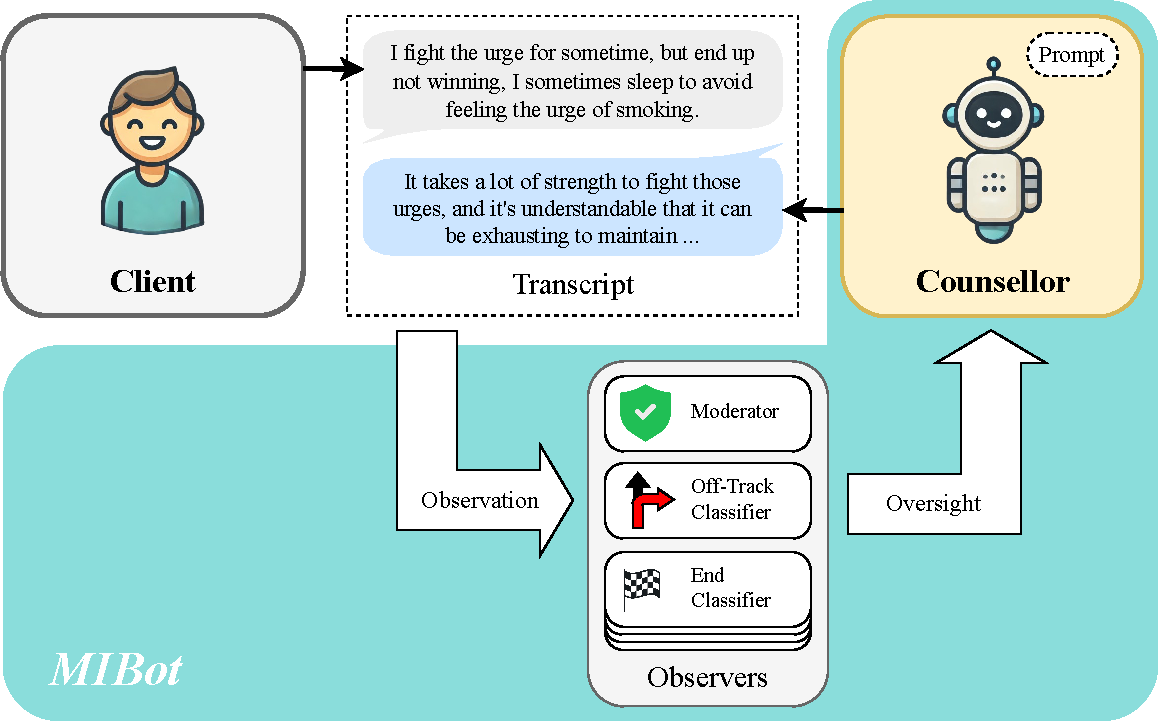
\includegraphics[width=0.8\linewidth]{fig/sysdiag.pdf}
    \caption{Overview of the \sysname system and observer agents.}
    \label{fig:system}
\end{figure*}
\input{latex/related_work}


\section{Chatbot Design Process}
\label{sec:design}


\textbf{Figure~\ref{fig:system}} illustrates an overview of the \sysname system. We first describe the elements of the MI counselling approach relevant to this paper.

\subsection{Motivational Interviewing}
\label{sec:MIdef}
Motivational Interviewing is a talk therapy approach for behaviour change, used by clinicians to help patients (called \emph{clients} in MI) move towards and make healthy behaviour changes. Its central strategy is to engage the client in contemplation around the behaviour and link change to their underlying values. The key to the MI approach is that clients themselves discover their motivation to change; the counsellors should neither be directive nor portray themselves as experts --- instead, they should guide the client without generating discord or increasing the ambivalence to change.

Typical conversational `skills' in MI include asking open-ended \emph{questions} around a behaviour, giving \emph{simple reflections} of client responses (restating these in different words) to encourage continued contemplation, linking the reflections to other relevant history or facts (\emph{complex reflections}) and offering \emph{affirmations} for positive accomplishments.

One key outcome of an MI conversation that the counsellor looks for is the kind of `talk' that the contemplation elicits from the client. \emph{Change Talk} refers to client utterances that indicate the client is contemplating or actively planning to change the behaviour. \emph{Sustain Talk} refers to utterances with reasons why it would be difficult for the client to change, or direct statements of the continuance of the habit. Ambivalent clients tend to oscillate between these two states, and thus appear stuck in their addiction. A core goal of MI is to help clients resolve this ambivalence. Successful MI results in a greater amount of Change Talk than Sustain Talk \cite{Apodaca2009}.


\subsection{Iterative Development of the Chatbot}
Our approach to building an automated counsellor chatbot is to begin with a single prompt of a state-of-the-art LLM, Open AI's GPT-4o model \citep{openai2024gpt4o}.  For consistency, all results presented in this paper are from a specific GPT-4o model, \texttt{gpt-4o-2024-08-06}.

Our research group is a collaboration of engineers and expert clinicians, the latter highly experienced in delivering MI counselling for smoking cessation.

The group used the following informal process to evolve the prompt for the counsellor chatbot: we began with a short, simple prompt (shown in Appendix~\ref{sec:initial_system_prompt}), which asks the model to use its own knowledge of MI. Then, sample conversations were generated between the chatbot and two different kinds of test clients: the first test client (a \emph{virtual} client) was a separate instance of the LLM instructed to play the role of a smoker. The prompt for the virtual client, including its ``backstory'' (a demographic specification and personal history), is given in Appendix~\ref{appendix:virtual_smoker_prompt}. The second test client was one of the human researchers role-playing as a smoker.

The resulting transcripts were then reviewed by the team of engineers and expert MI clinicians and researchers, who identified issues in bi-weekly meetings. The discussions would lead to an improved prompt to address the issues. Each revised prompt was tested with several more counsellor-test-client conversations to see if the improvement was successful.

The list below gives the set of the most important improvements made to the prompt, linked to specific lines of the final prompt (given in Appendix~\ref{sec:system_prompt}) that were changed to make that improvement.

\begin{enumerate}[itemsep=0pt, parsep=0pt]
    \item \textbf{Appropriate utterance length}: It was observed that the chatbot had a tendency to be quite verbose, which would make it sound unnatural and overwhelming to the client. The prompt was modified (in lines 2-3 of Appendix~\ref{sec:system_prompt}) to address this.

    \item \textbf{Accessible Language}: To make \sysname accessible to users from diverse educational and socioeconomic backgrounds, it was instructed to use simple language, avoid complex terminology, and adapt to the client's language. The prompt was modified (in line 2 of Appendix~\ref{sec:system_prompt}) to address this.

    \item \textbf{Avoiding assumptions about nicotine use}: It was observed that the chatbot sometimes made a premature assumption about the nature and extent of the client's smoking. The MI clinicians suggested that a counsellor should enter the conversation with an open mind and let the client describe the amount of smoking. The prompt was modified (in line 6 of Appendix~\ref{sec:system_prompt}) to address this.

    \item \textbf{Improved conversation pace:} The chatbot had the tendency to move into the conversational topic of smoking quickly and put insufficient effort into building rapport with the client. Clinicians emphasized the need to start conversations with icebreakers to create a comfortable environment for the client. The prompt was modified to reflect this in lines 1 and 7.

    \item \textbf{Appropriate timing of the planning phase:} Planning is a crucial step in MI, in which clients begin to think through concrete ideas on how they would bring change to their behaviour. However, guiding clients to begin planning prematurely can be counter-productive and drive them away from change. The prompt was modified in lines 9-13 to give instructions on how and when to move towards the planning phase. A key understanding here is to wait until the client demonstrates a reduced amount of sustain talk.
\end{enumerate}


These iterative discussions continued until the team was (informally) satisfied with the quality and MI adherence of virtual/role-played conversations.


\subsection{Observer Agents}
In addition to the primary counsellor agent, to ensure the chatbot could be deployed safely for end users, we developed observer agents to monitor the conversations between the chatbot and the client. Each observer is built using a prompted GPT-4o instance,
tasked with reviewing specific aspects of the ongoing conversation and can intervene when necessary, as described below.

\subsubsection{The Moderator}
The \textit{moderator} reviews the counsellor's most recent utterance and determines whether it could potentially harm the client. While OpenAI's internal guardrails \citep{openai_safety_update_2024} are highly effective at preventing some forms of harmful content, they do not safeguard against counterproductive counsellor utterances. We designed this observer to have high sensitivity (and, consequently, a high false positive rate). If the moderator deems that the counsellor's utterance is potentially encouraging self-harm (which might include a suggestion to actually smoke), the system re-generates the counsellor's utterance, which is again checked. This process is repeated up to a maximum of five attempts or until the moderator deems the latest utterance ``acceptable''. In all experiments described below, the re-generated counsellor utterance succeeded within four generation attempts and never failed to produce an acceptable utterance.

\subsubsection{Off-Track Conversation Classifier}
We were concerned that some of our participants might intentionally steer the conversation far off from the topic of smoking.
We built a classifier to monitor conversations in real-time to detect if the client is deliberately steering the conversation off-track. Unlike the moderator observer, this classifier was prompt-engineered for a low false positive rate to give the benefit of the doubt to the client. The purpose of this classifier was to identify participants who were not engaging in a serious conversation for removal from the dataset. In an actual deployment, this observer could be used to trigger the end of the conversation.

\subsubsection{End Classifier and Conversation Termination}
The intent to end a conversation can arise from either the client or the counsellor. To ensure the conversation transitions smoothly to an ending and the post-conversation survey, we designed an \textit{end classifier} that monitors the dialogue in real-time and determines if the counsellor or client wishes to finish. If so, the counsellor is instructed to summarize the conversation (a typical MI practice) and ask if the client wishes to continue. If the client does wish to continue, then the conversation is resumed.

\section{Feasibility Study with Human Smokers}
\label{sec:feasability_study}
\subsection{Participant Recruitment}
\label{sec:recruitment}
A total of 106 English-speaking participants were recruited to evaluate the capability of \sysname through the Prolific (www.prolific.com) online behavioural research platform \cite{peer2017beyond}. The criteria for inclusion in the study were that participants must be fluent in English, had a high approval rate on prior tasks performed on the Prolific platform, and must be current smokers of at least five cigarettes per day. This group was also filtered from a larger group of 159 participants to select those who exhibited low confidence that they will succeed in quitting\footnote{
As the goal of MI is to resolve ambivalence, those who are very confident in succeeding in quitting are already in the state MI is meant for. So, we only include participants who exhibit low confidence ($\leq 5$ ). We also include `discordant' participants who have high confidence relative to their importance (confidence $>$ 5 and confidence $-$ importance $< 5$) as they don't think it is important to quit and, therefore, need MI-style counselling.}. Finally, the recruitment was set to enrol equal numbers of male and female participants. The exact balance was affected by the above filter, and so the final sex proportion was 54\% females and 46\% males. Participant ages ranged from 22–77 years old, with a median of 38 years (mean=40, SD=13). The median and mean time taken to complete the conversational part of the study was 19 minutes (SD=9). Appendix~\ref{appendix:participant_demographics} provides more details on participant demographics.

\subsection{Study Design}
\label{sec:evaluation}
The study design followed a pattern commonly employed in MI research (e.g., \citealp{Valanis2001, doi:10.15288/jsads.2009.s16.106, 10.1093/alcalc/agw047, browne2022motivation, james2021improving}) and therapeutic chatbot evaluations (e.g., \citealp{info:doi/10.2196/49132, He2022}). Participants in our study were taken through the following four steps (a diagram view is available in Appendix~\ref{app:stud_flow}):\vspace{-0.2em}

\begin{enumerate}
[itemsep=1pt, parsep=0pt]
    \item In a \textbf{pre-conversation survey}, participants rated themselves on the \textbf{readiness ruler} survey, which is often used in behaviour change \cite{rollnick1992development}. These are three numerical questions (scored from 0 to 10) measuring how \textit{important} it is for the participant to quit, how \textit{confident} they are that they will succeed, and how \textit{ready} they are to quit right now. The specific survey is given in Appendix~\ref{appendix:readiness_rulers}.

    \item Participants then engaged in a \textbf{conversation} with the counsellor chatbot described in Section~\ref{sec:design}, through a text-based interface.

    \item \textbf{Post conversation}, participants completed the readiness rulers again, provided feedback on the conversation itself, and responded to the CARE survey (\citealp{10.1093/fampra/cmh621, Bikker2015}), which measures their perceived empathy of the counsellor and is used to evaluate human clinical practitioners. It has 10 questions rated on a scale from 0 to 5 each (Appendix~\ref{appendix:care_questionnaire}).

    \item \textbf{One week after} the conversation, participants again completed the readiness ruler and indicated if they made any quit attempts or changes in smoking habits.
\end{enumerate}

It has been shown that readiness to quit predicts quitting (\citealp{Boudreaux2012,10.1093/alcalc/agw047}), and the most predictive part of the ruler is the self-reported \textbf{confidence} to succeed, which we used as our primary metric for therapeutic effectiveness \citep{Gwaltney2009-wj,Abar2013}.


\subsection{AutoMISC: Assessment of Counsellor and Client Language}
\label{sec:automisc}
\label{sec:automisc_val}

In addition to the participant-reported effectiveness metrics described above, it is important to evaluate whether the counsellor's generated text adheres to the MI methodology to establish clinical validity. Assessment of client text can also offer direct evidence of success or failure in the counselling session, as discussed in Section~\ref{sec:MIdef}. Since we wanted to assess both counsellor and client utterances, we chose to use the original MI assessment rubric, the Motivational Interviewing Skills Code (MISC) version 2.5 \cite{MISC}.

MISC classifies each \emph{utter\-ance} into pre\--defined categories based on the counsellor and client behaviours. Counsellor codes include the skills described in Section~\ref{sec:MIdef}, among others. MISC also provides transcript-level summary scores computed by aggregating the utterance-level annotations. Metrics to assess counsellor adherence to MI include \textbf{Percentage MI-Consistent Responses (\%MIC)}, where higher values indicate greater adherence, and \textbf{Reflection-to-Question Ratio (R:Q)}, where values between 1 and 2 are considered indicative of proficiency \cite{moyers2016miti}. For client language, the \textbf{Percentage Change Talk (\%CT)} is used, with higher values associated with improved behavioural outcomes \cite{Apodaca2009}.

As described in Section~\ref{sec: BackgroundAutomEval}, it is difficult to label transcripts manually, so we developed \textbf{AutoMISC} to automate this process. AutoMISC processes a counselling session transcript by first parsing each speaker's turn into \textit{utterances} (individual units of thought). This is done by a separate prompted instance of GPT-4o, as is the next step: each counsellor utterance is classified into one of MI-Consistent (MICO), MI-Inconsistent (MIIN), Reflection (R), Question (Q), or Other (O).
We found that including five previous conversation turns to classify the current utterance gave enough context to ensure high accuracy.
Each client utterance is classified into one of Change Talk (C), Sustain Talk (S) or Neutral (N). These can then be computed into the transcript-level summary scores described above. The prompts for each instance of GPT-4o are listed in Appendix~\ref{appendix:automisc_prompts}.

To validate the reliability of AutoMISC, its annotations were compared against four human annotators: two expert MI clinicians and two non-expert team members. Each annotator manually labelled ten of the 106 transcripts, a total of 821 utterances (580 from the automated counsellor, 241 from clients). The inter-rater agreement was measured pairwise using Cohen's $\kappa$ and for the group using Fleiss' $\kappa$. The overall Fleiss' $\kappa$ was \textbf{0.68} for counsellor codes and \textbf{0.67} for client codes, which indicates substantial agreement \cite{cohenrange}.  Appendix~\ref{appendix:automisc_val} provides more detail on the inter-rater agreement.
\section{Results}
\label{sec:results}


\subsection{Effect of Conversation on Participants' Readiness to Quit Smoking}
\label{sec:result_readiness}

\begin{table}[phtb!]
  \centering
  \renewcommand{\arraystretch}{0.9}
  \setlength{\tabcolsep}{3pt}
  {
  \begin{tabular}{
  @{} p{0.23\linewidth}
  p{0.23\linewidth}
  p{0.23\linewidth}
  p{0.23\linewidth} @{}
  }
    \toprule
    \textbf{Average} &
    \textbf{Average} &
    \textbf{Average} &
    \textbf{Average $\Delta$}  \\

    \textbf{Before} &
    \textbf{After} &
    \textbf{1-Week} &
    \textbf{(1-Week }  \\

    \textbf{Conv} &
    \textbf{Conv} &
    \textbf{After} &
    \textbf{$-$ Before)}  \\

    \midrule\vspace{-4pt}\\[-8pt]

    \multicolumn{4}{@{}l}{\textit{\textbf{Importance}}} \\
    5.7 (2.6) & 6.3 (2.9) & 6.1 (2.7) &  0.5 (1.7)$^*$  \\

    \arrayrulecolor{gray!50}\midrule\vspace{-4pt}\\[-8pt]

    \multicolumn{4}{@{}l}{\textit{\textbf{Confidence}}} \\
    2.8 (2.0) & 4.6 (2.6) & 4.5 (2.7) & 1.7 (2.4)$^{**}$  \\

    \arrayrulecolor{gray!50}\midrule\vspace{-4pt}\\[-8pt]

    \multicolumn{4}{@{}l}{\textit{\textbf{Readiness}}} \\
    5.2 (2.8) & 5.9 (2.8) & 5.5 (3.0) &  0.3 (2.4)$^\dagger$ \\

    \arrayrulecolor{black}\bottomrule
  \end{tabular}}

  \caption{Average (SD) of Readiness Ruler Survey on Importance, Confidence, and Readiness to quit smoking. Statistical significance using Wilcoxon signed-rank test. $^*$: $p < 0.005$, $^{**}$: $p < 0.001$, $^\dagger$: $p = 0.22$.}

  \label{table:readiness_ruler}
\end{table}

Recall from Section~\ref{sec:evaluation} that the 106 human participants in the study completed the readiness ruler survey on three occasions: just before the conversation with the chatbot, just after it, and one week later. The primary measure of effectiveness is the difference in confidence from before the conversation to one week later, as this is the most predictive of downstream quitting success \citep{Gwaltney2009-wj}.
\textbf{Table~\ref{table:readiness_ruler}} presents data at those points in time for the three readiness rulers: importance, confidence, and readiness. It shows a significant increase in confidence of +1.7 on the ten-point scale.

As a point of reference, our previous work, \oldsysname \citep{info:doi/10.2196/49132}, which used a hybrid of scripted questions and LLM-generated reflections, reported an average change in confidence of +1.3. While that result is not directly comparable to the present one, both works recruited a similar number of low-confidence participants but at a different time and with a different starting average confidence.

We can also compare the week-later change in confidence to that achieved by human counsellors. \citet{rachelthesis} found that participants' confidence increased by +2.5 points after five MI sessions over a ten-week period.

\textbf{Figure~\ref{fig:confidence_change_dist}} presents the distribution of week-later changes in confidence scores. Notably, 28\% of  participants did not change their confidence level, but a substantial number (around 60\%) showed a positive change in confidence. Roughly 12\% decreased their confidence by 1-2 points, and a larger decrease was observed in 2\% of the participants.

\textbf{Table~\ref{table:readiness_ruler}} also shows that there was a significant change in the participants' view of the importance of quitting, with an average increase of +0.5, exhibiting the chatbot's effectiveness. The change in readiness was not statistically significant.

Finally, \textbf{Table~\ref{table:demographics_wise_conf}} in Appendix~\ref{appendix:demographics_wise_confidence} shows that baseline confidence levels and one-week changes varied by demographic group. Younger participants, for instance, started with a higher average confidence of 3.7 and saw a larger increase of +1.9 over the week.


\begin{figure}[!tphb]
\centering
  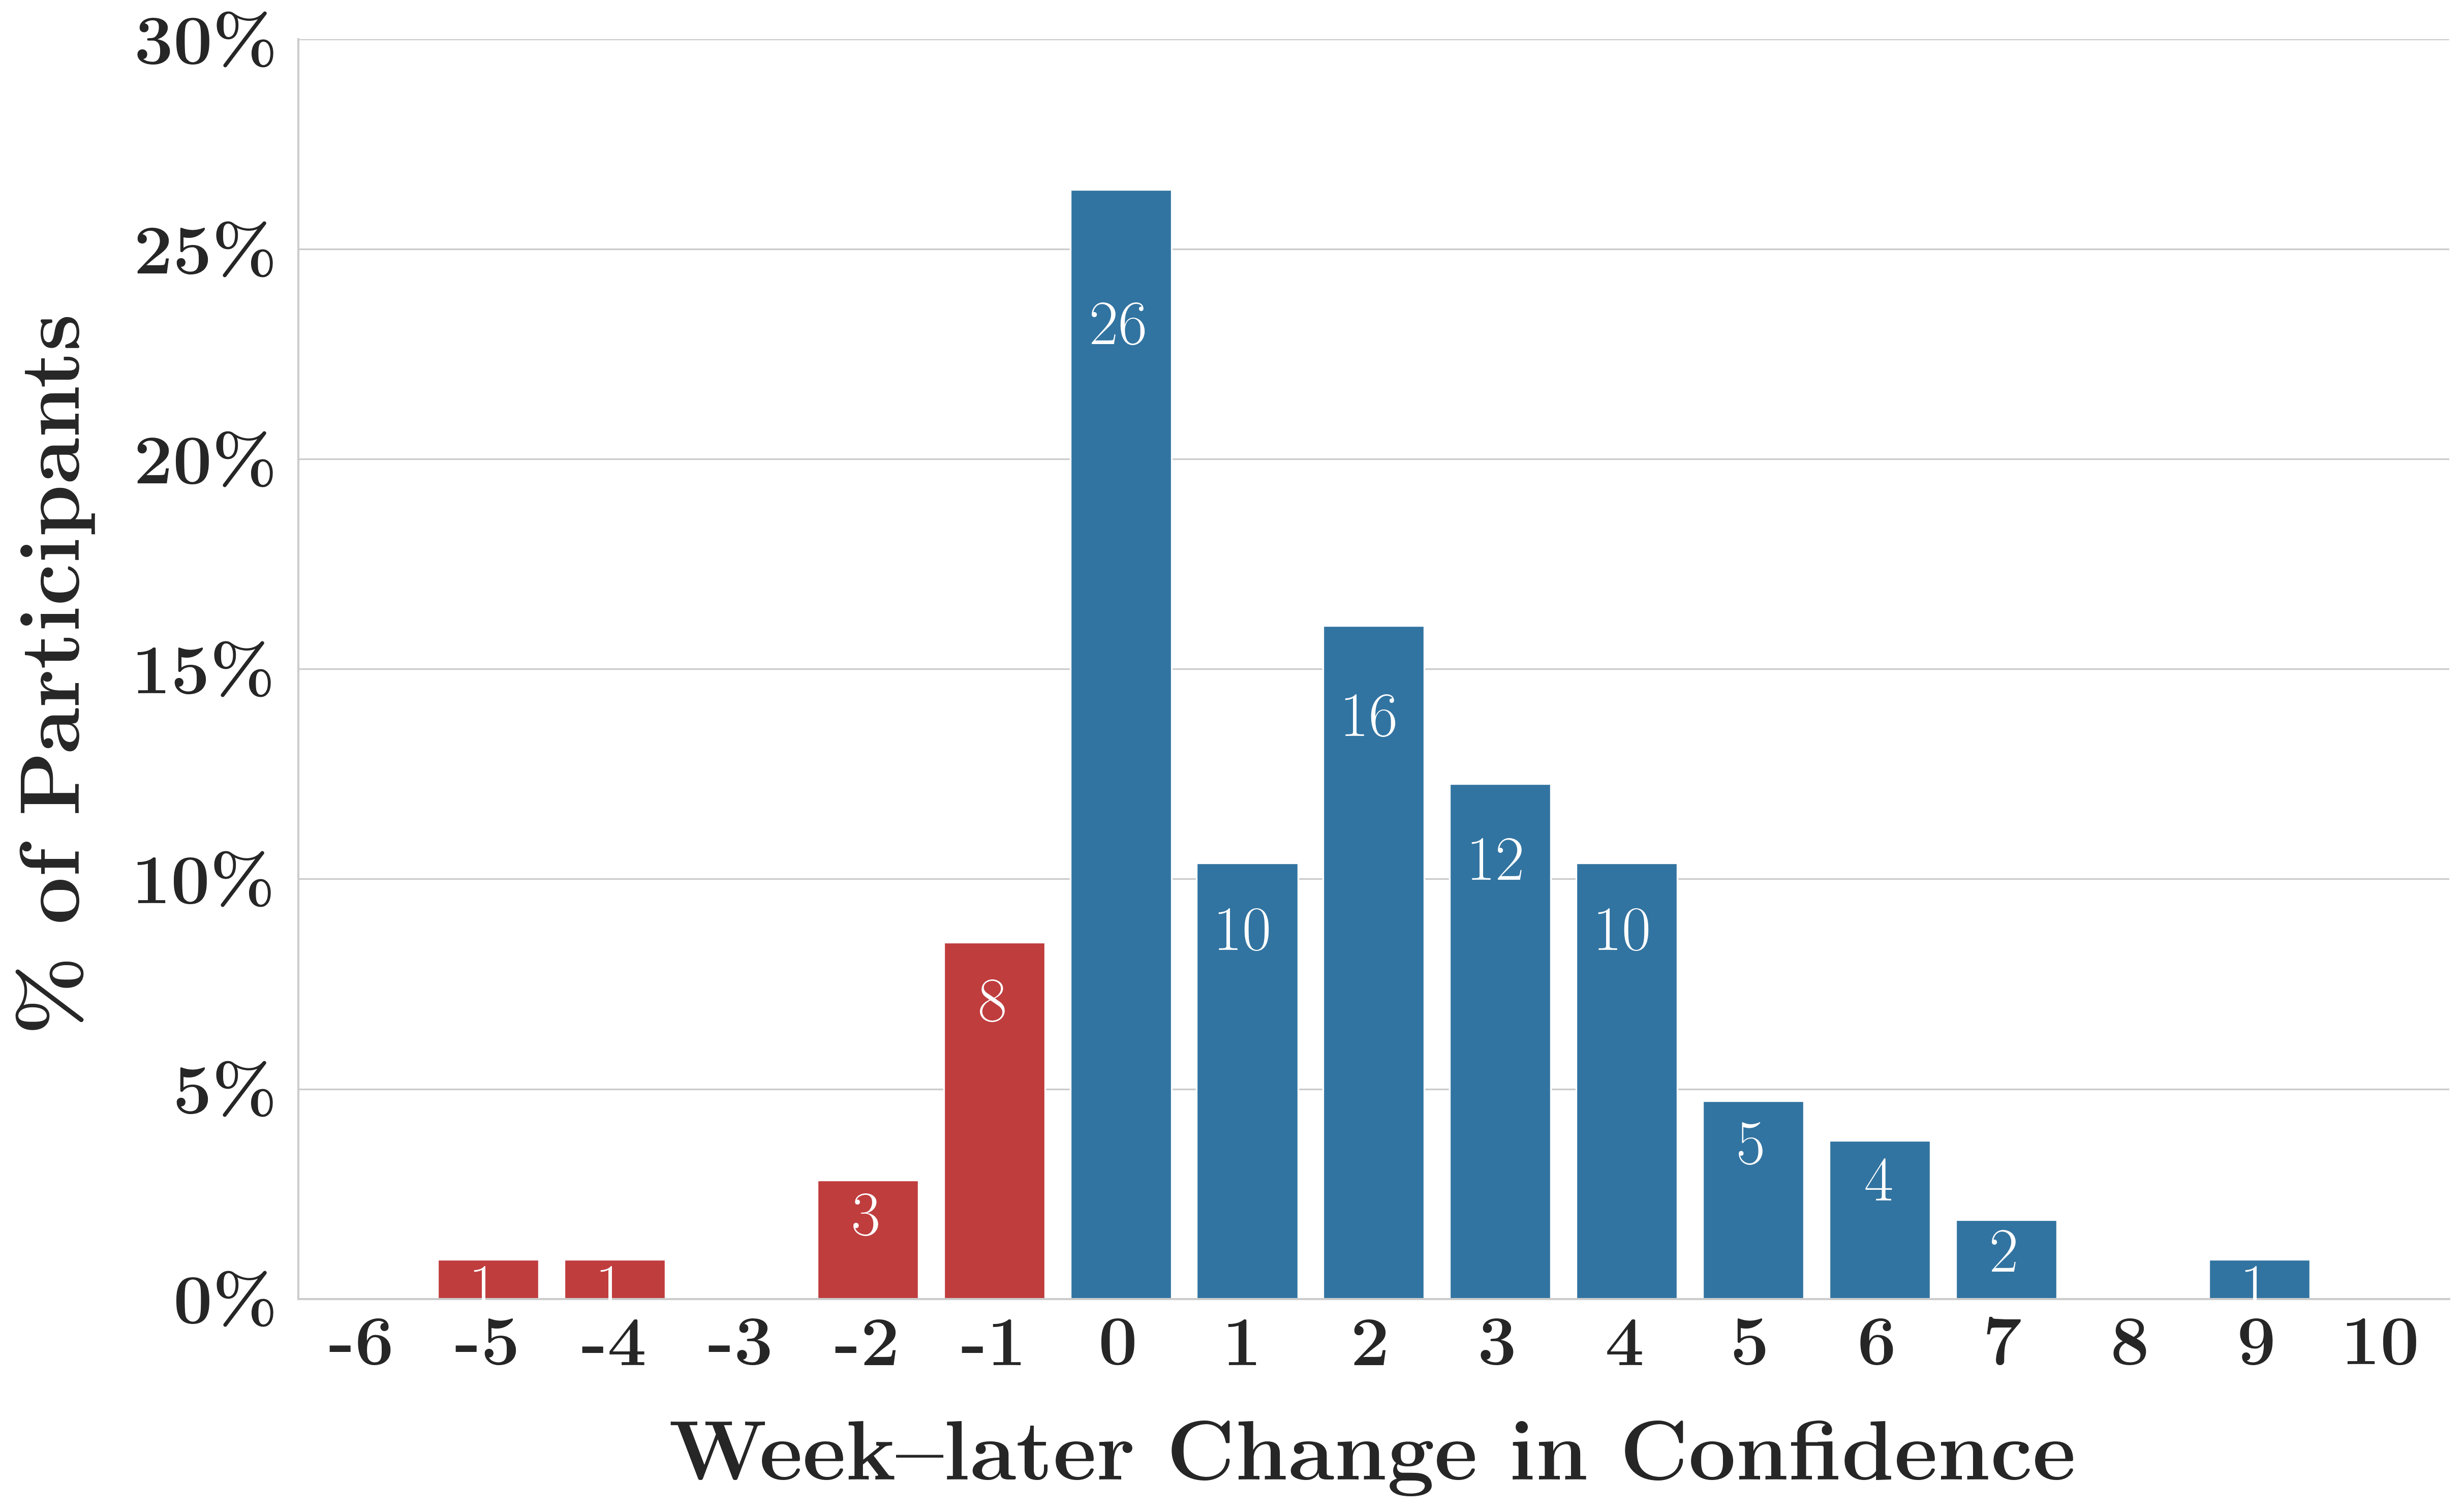
\includegraphics[width=\linewidth]{fig/2024-11-14-MIV6.3A-2024-11-22-MIV6.3A_ruler_deltas_delta_with_week_later_keep_high_conf_False_change.png}
  \caption {Distribution of Change in Confidence (1-Week Later $-$ Before Conversation).}
  \label{fig:confidence_change_dist}
\end{figure}

\begin{figure*}[htpb!]
    \centering
    \begin{subfigure}[b]{0.32\textwidth}
        \centering
        \captionsetup{justification=centering}
        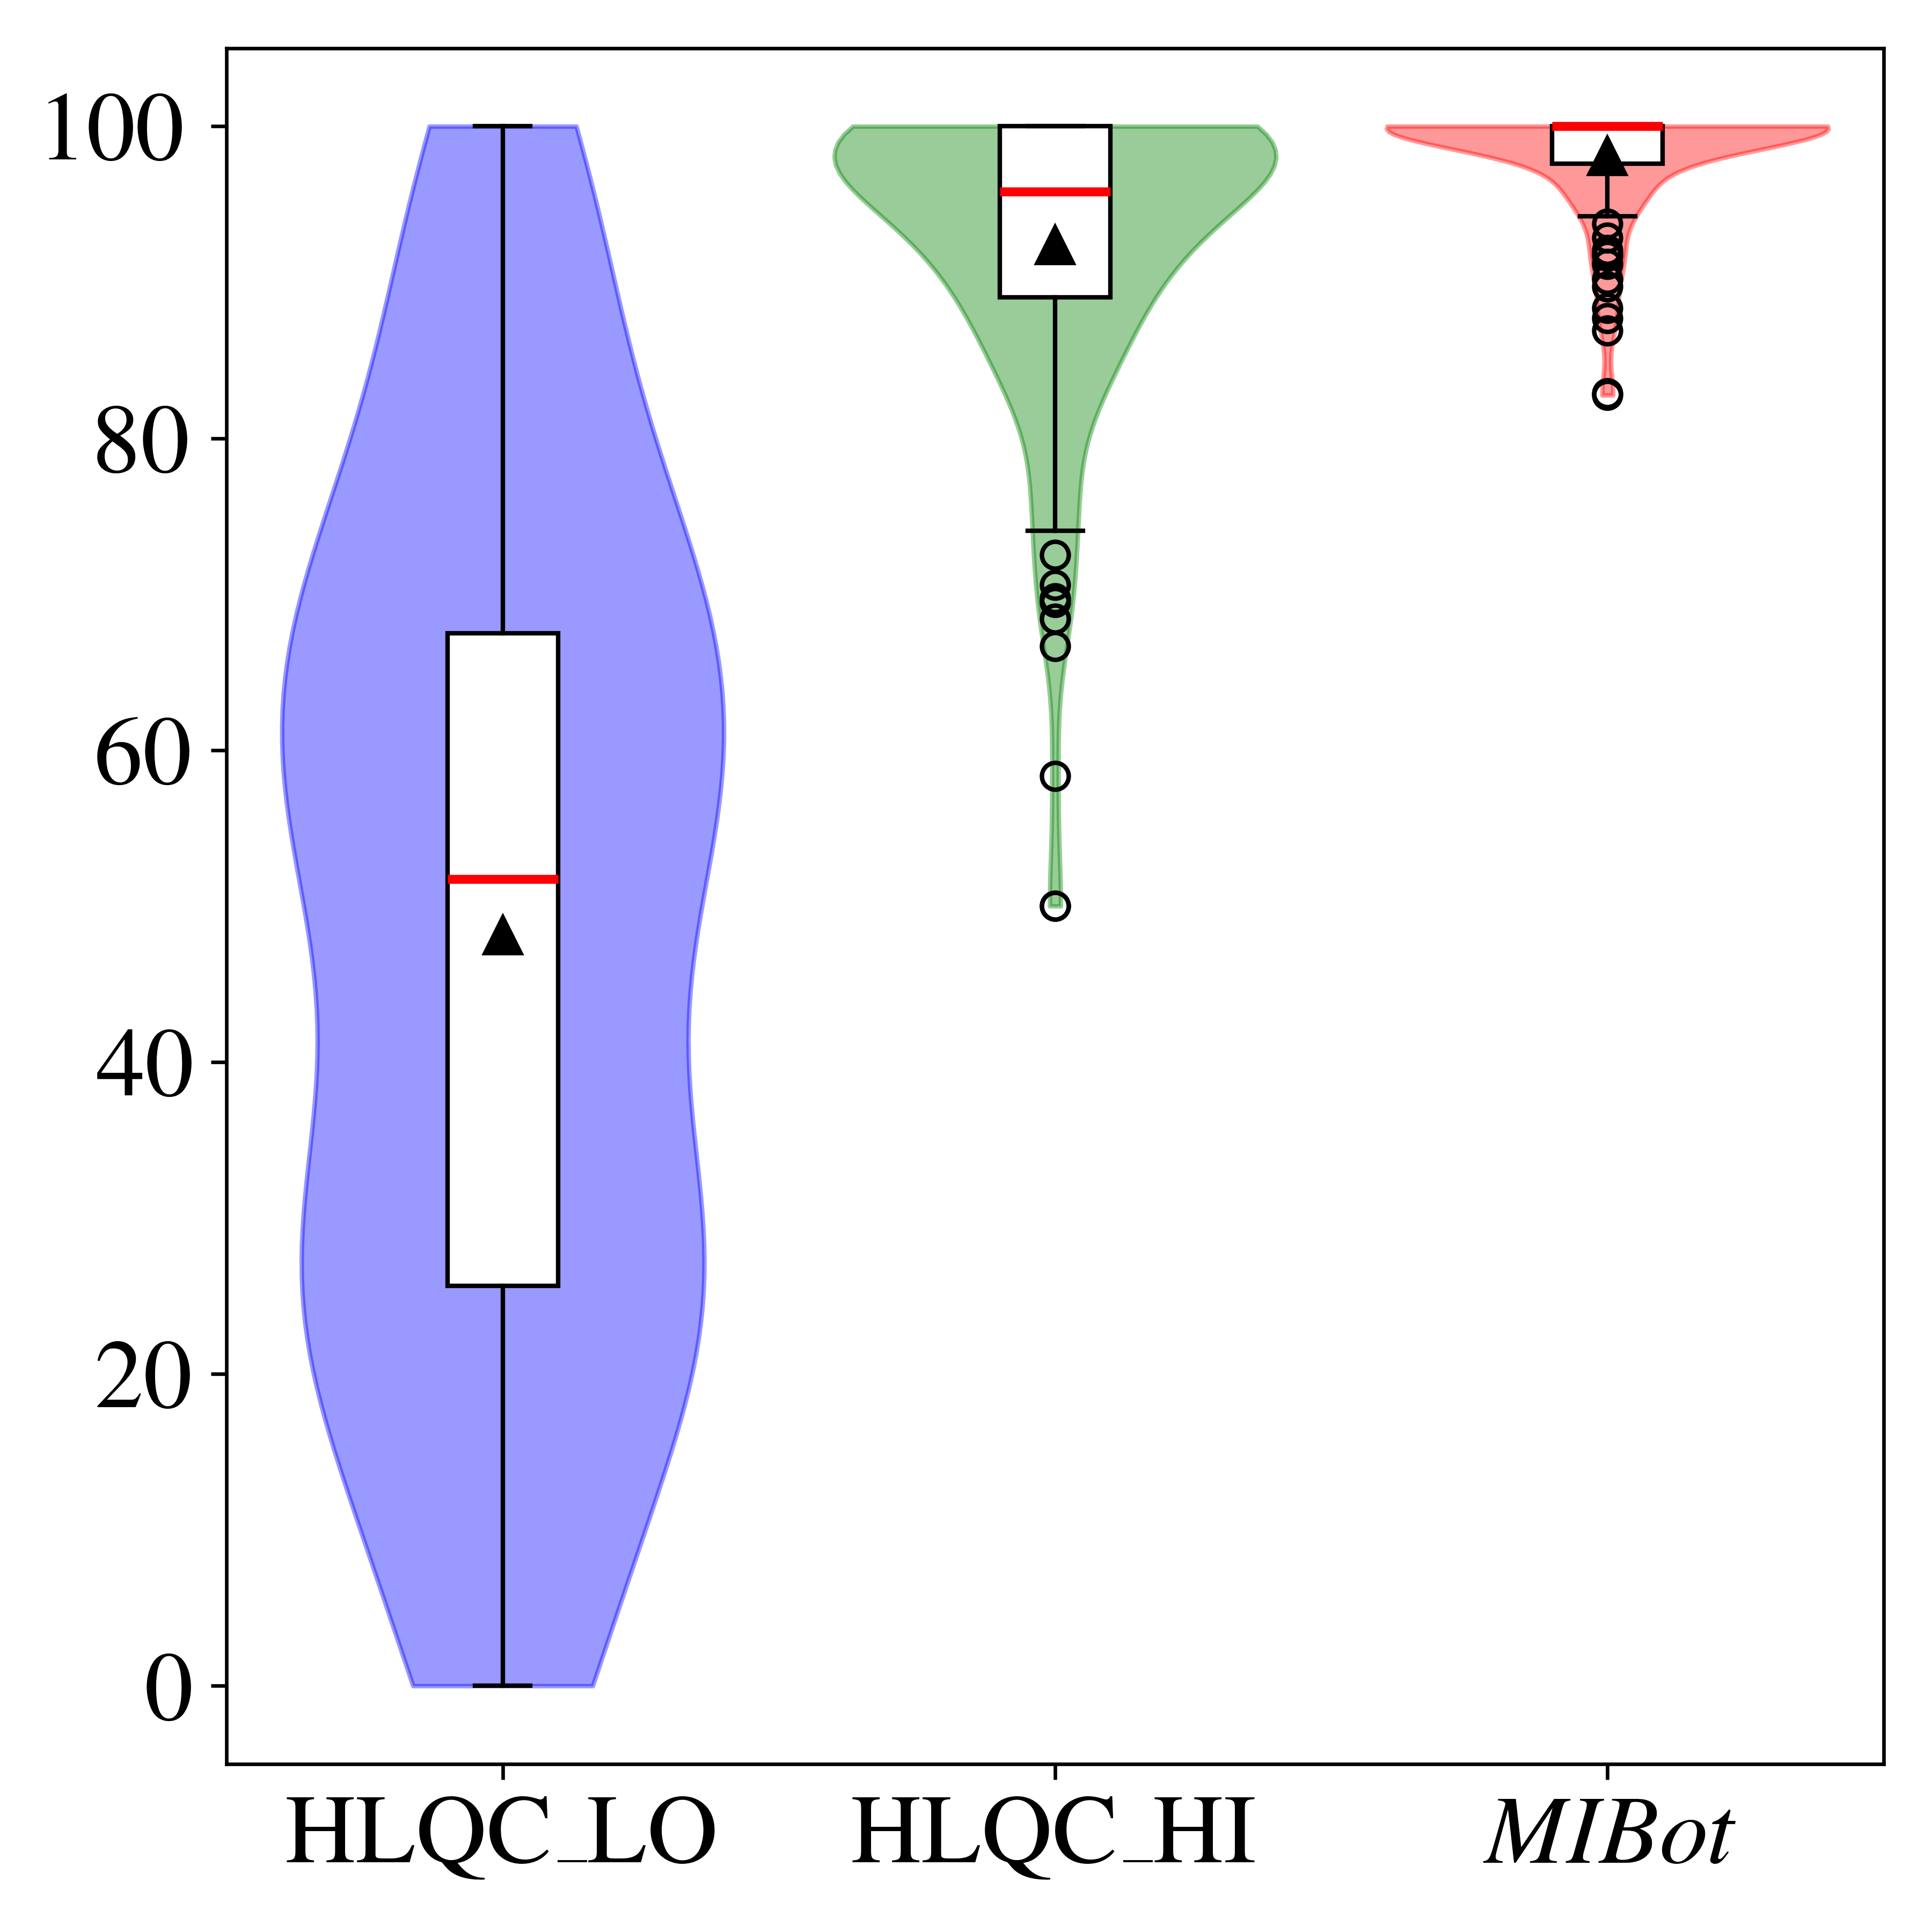
\includegraphics[width=\textwidth]{fig/mic.png}
        \caption{Percentage MI-Consistent Responses\\(\%MIC)}
        \label{fig:mic}
    \end{subfigure}
    \hfill
    \begin{subfigure}[b]{0.32\textwidth}
        \centering
        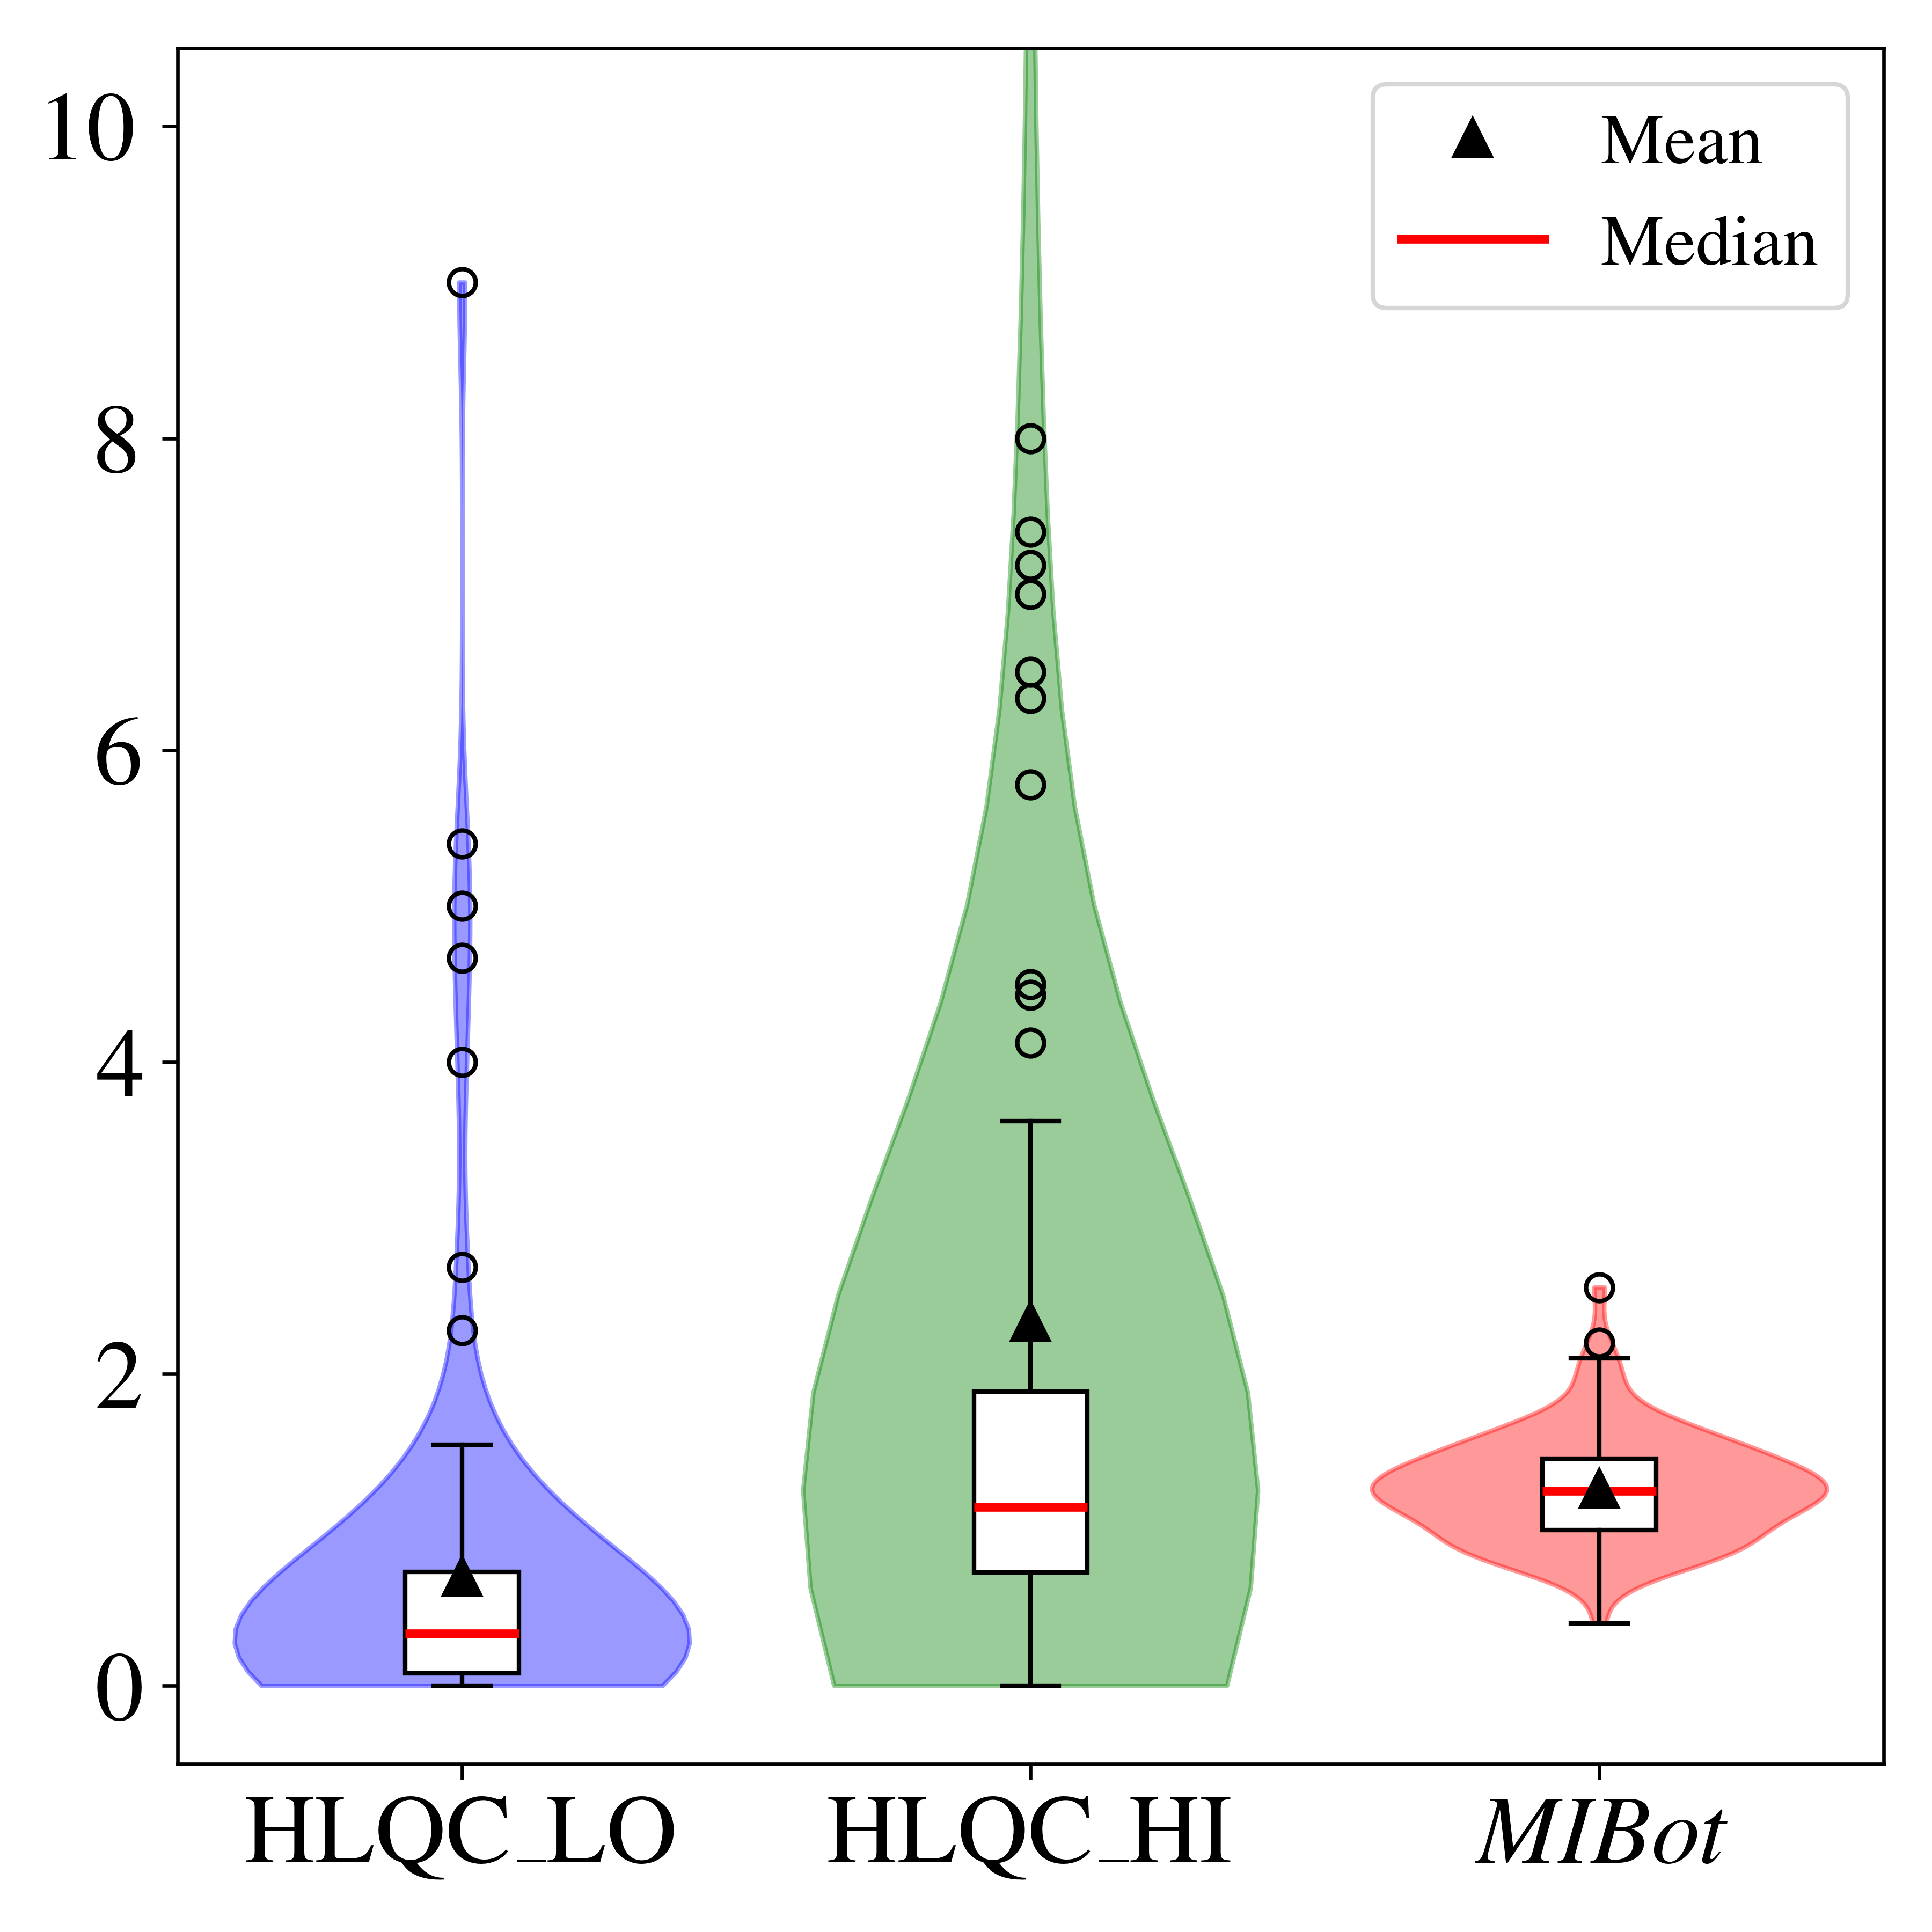
\includegraphics[width=\textwidth]{fig/rq.png}
        \caption{Reflection to Question Ratio \\(R:Q)}
        \label{fig:rq}
    \end{subfigure}
    \hfill
    \begin{subfigure}[b]{0.32\textwidth}
        \centering
        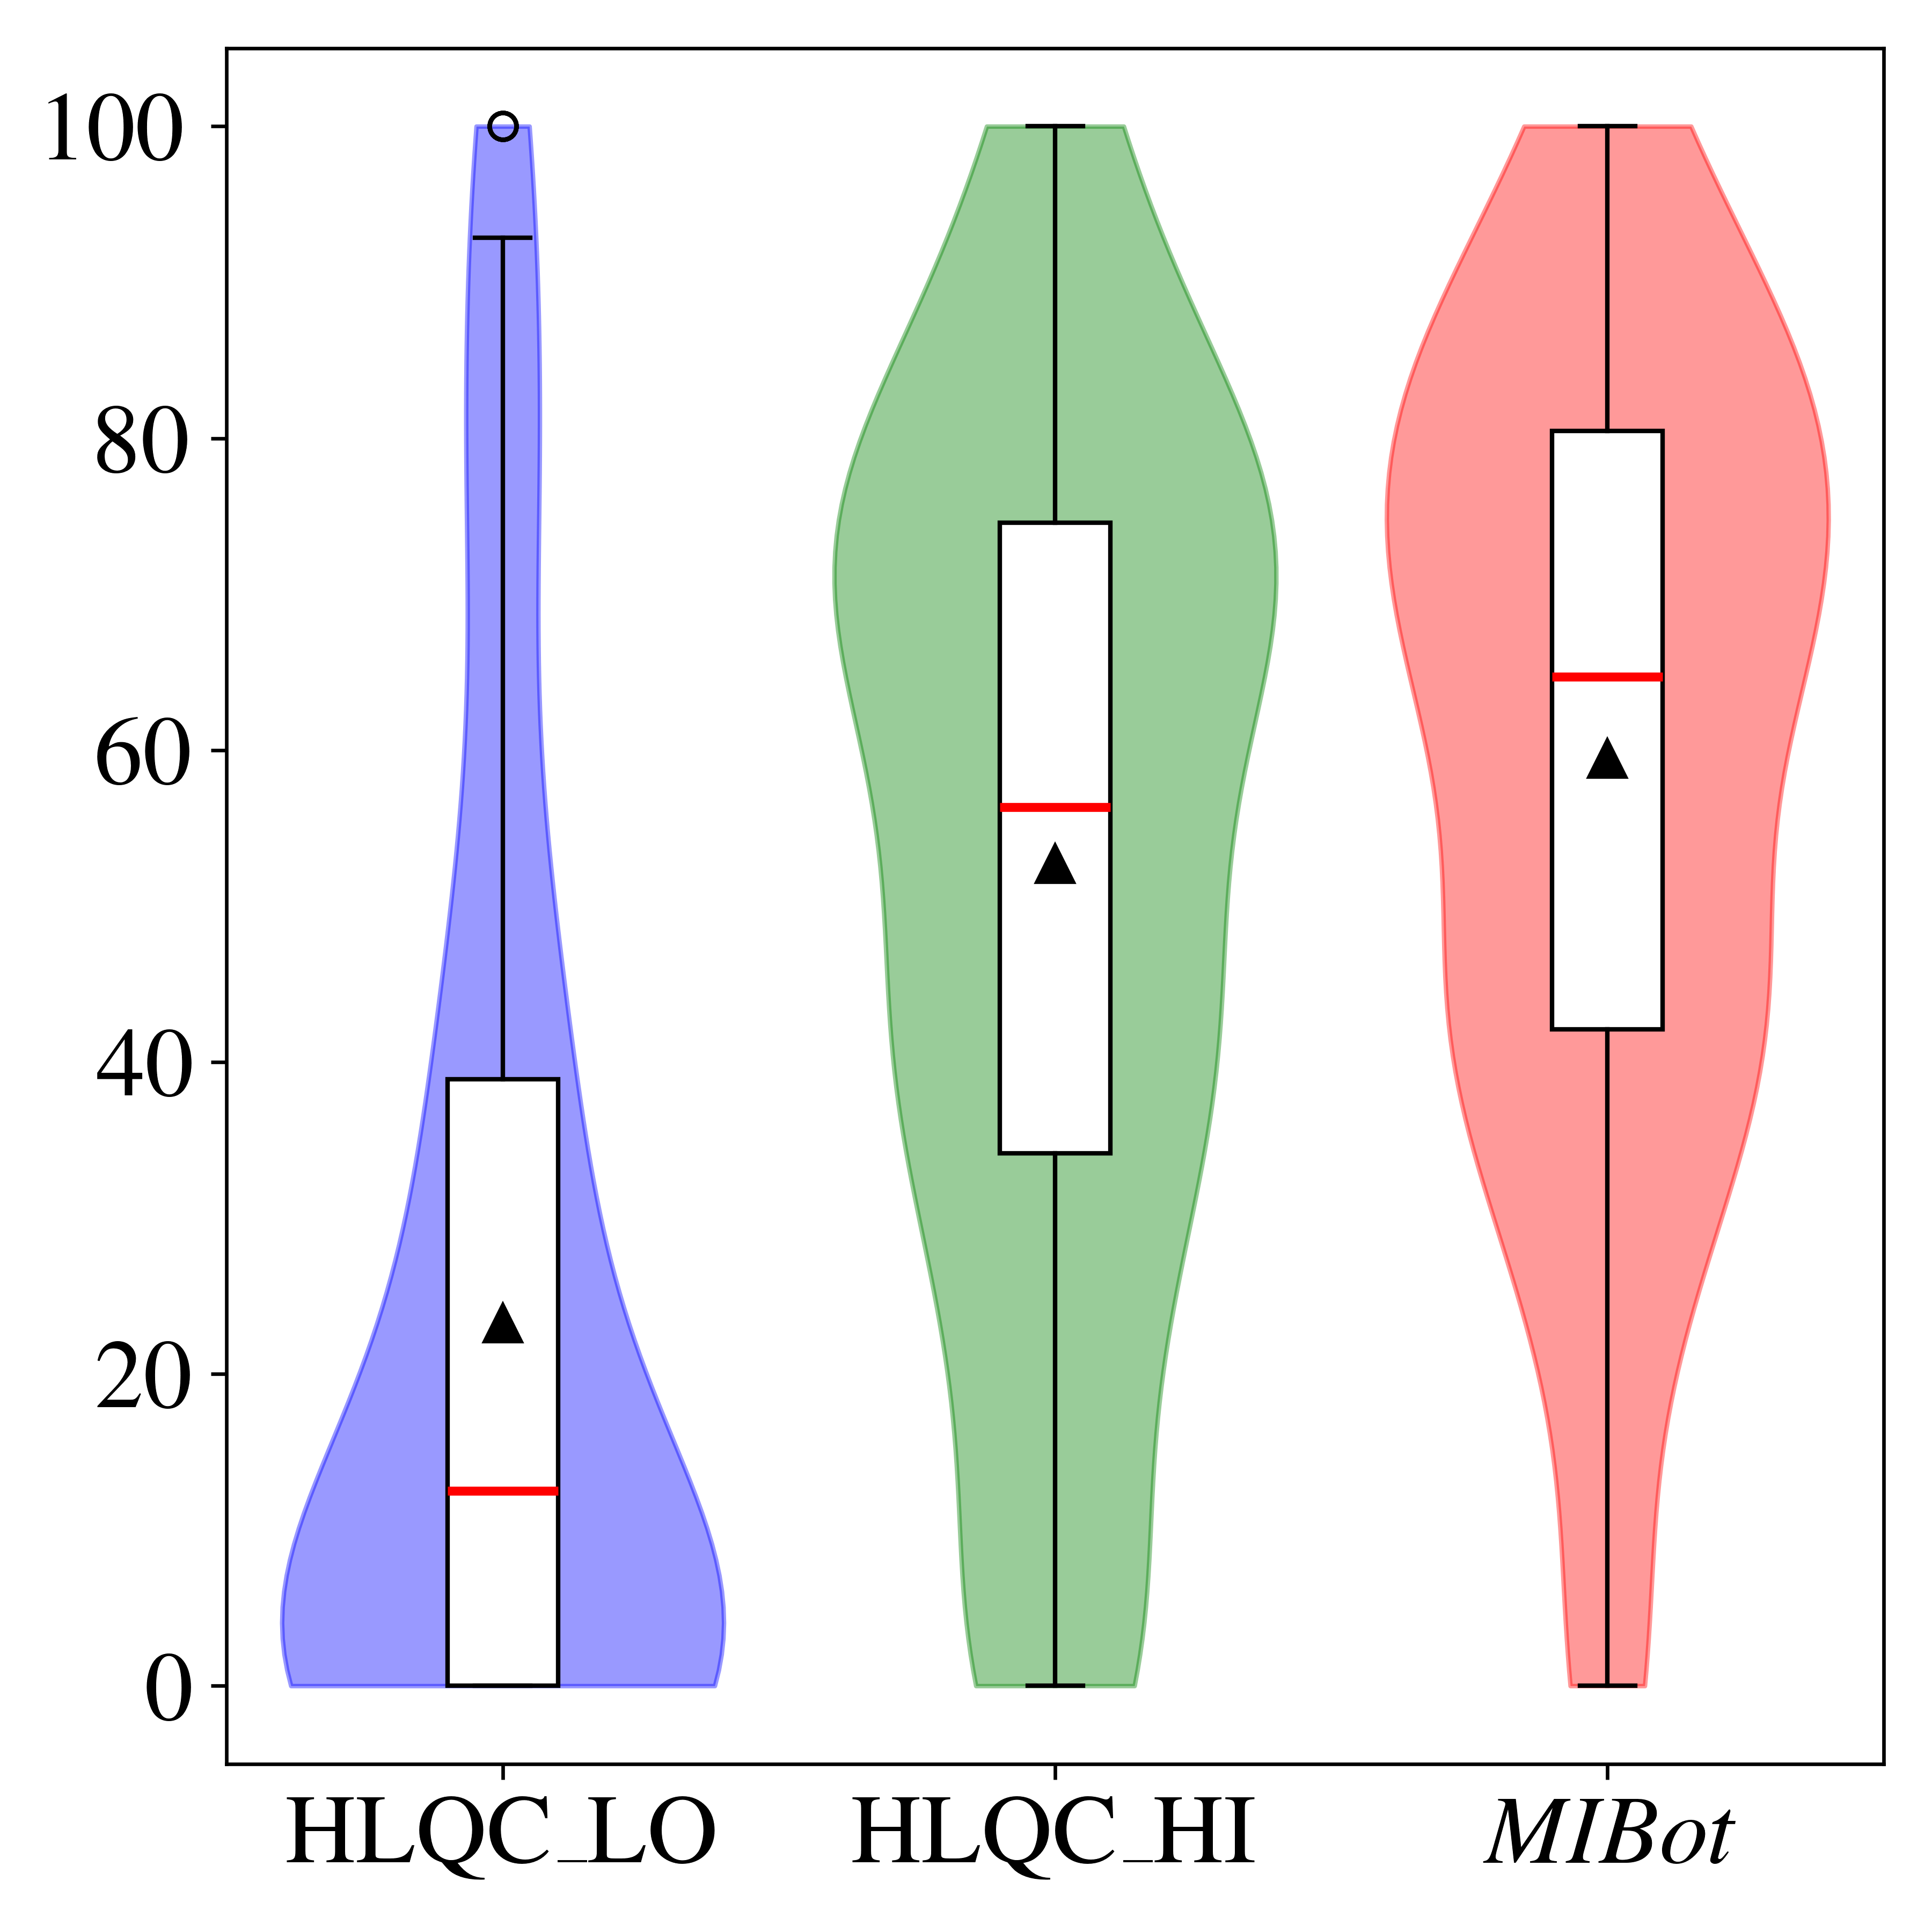
\includegraphics[width=\textwidth]{fig/ct.png}
        \caption{Percentage Client Change Talk \\(\%CT)}
        \label{fig:ct}
    \end{subfigure}
    \caption{Comparison of MISC summary score distributions across datasets.}
    \captionsetup{justification=justified}
    \label{fig:violin_box_plots}
\end{figure*}


\subsection{CARE Metric for Empathy}
\label{sec:CARE}
Each participant rated the perceived empathy of the chatbot on the CARE scale (\citealp{10.1093/fampra/cmh621}).
\textbf{Table~\ref{table:care}} presents the mean CARE scores for this work (\sysnamewithv) and our previous work, \oldsysname \citep{info:doi/10.2196/49132}. The fully generative \sysnamewithv is significantly more empathetic than a partially scripted and partially generative \oldsysname. Notably, 11\% of the participants gave \sysnamewithv a perfect score of 50, substantially higher than the 3\% achieved by \oldsysname. Compared to trained human counsellors, however, this number is quite low, as \citet{Bikker2015} found that nurses scored an average of 46 on the CARE metric, with 48\% achieving a perfect score of 50.
\begin{table}[htpb]
  \centering
  \setlength{\tabcolsep}{3pt}
  \renewcommand{\arraystretch}{0.9}
   {
  \begin{tabular}{@{}l@{\hspace*{3mm}}rr@{}}
    \toprule
    \textbf{} & \textbf{CARE} & \textbf{\% Perfect} \\
    \textbf{} & \textbf{Score} & \textbf{Score} \\
    \specialrule{0.4pt}{1pt}{1pt}
    \oldsysname & 36 & 3 \\
    \sysnamewithv & 42  & 11 \\
    Humans$^*$  & \textbf{46} & \textbf{48} \\
    \bottomrule
  \end{tabular}}
  \caption{Average CARE scores and (\%) perfect scores for \oldsysname, \sysnamewithv (present work) and $^*$typical human healthcare professionals \citep{Bikker2015}.
  }
  \label{table:care}
\end{table}


Appendix~\ref{appendix:CAREdist} provides the distribution of CARE scores among participants and question-wise mean CARE scores. The chatbot performed poorly on questions, such as ``How well did the chatbot show interest in you as a whole person?'' and ``How well did it assist in making a plan of action with you?''. The poor performance on some questions may be due to the chatbot's lack of emotional intelligence \citep{sabour-etal-2024-emobench} or collaboration skills \citep{yang-etal-2024-human}.

The general post-conversation survey showed that 92\% of participants enjoyed the experience, while 66\% found the interactions helpful.

\subsection{Adherence to MI}
\label{misc_summary_metrics}

The AutoMISC assessment tool, described in Section~\ref{sec:automisc_val}, was applied to the 106 transcripts from the study. To provide a point of comparison for the MISC summary metrics, we also ran it on the \textbf{High\-Low\-Quality\-Counselling (HLQC)} dataset \cite{perez-rosas-etal-2019-makes}, a publicly available\footnote{ \url{https://lit.eecs.umich.edu/downloads.html}} corpus of transcribed MI counselling demonstrations. It was designed to support the development of  ``data-driven methods for the automatic evaluation of counselling quality.'' The HLQC dataset comprises 155 high-quality (HLQC\_HI) and 104 low-quality (HLQC\_LO) transcripts sourced from public websites. We computed summary scores separately for these subsets and then compared \sysname's summary metrics against those of both HLQC\_HI and HLQC\_LO. \textbf{Table~\ref{table:mi_metrics_summary}} summarizes the computed MISC metrics across datasets. It shows that a very high fraction of the chatbot counsellor utterances are MI-compliant (\%MIC in the table), exceeding those in the high-quality dataset with less variance. The chatbot's Reflection to Question Ratio (R:Q) falls between that of the high- and low-quality datasets and aligns with the 1-2 range recommended in the MISC rubric. Finally, the fraction of participant utterances classified as \textit{change talk} is higher than in the high-quality dataset.


\begin{table}[thpb!]
  \centering
  \setlength{\tabcolsep}{4pt}
  \renewcommand{\arraystretch}{0.9}
  {
  \begin{tabular}{@{}llr@{}}
    \toprule
    \textbf{Metric} & \textbf{Dataset} & \textbf{Mean (SD)} \\
    \specialrule{0.4pt}{1pt}{1pt}

    \multirow{3}{*}{\textbf{\%MIC}}
    & HLQC\_LO & 48 (27.9) \\
    & HLQC\_HI & 92 (9.8) \\
    & \sysname & \textbf{98 (3.6)} \\

    \arrayrulecolor{gray!50}\midrule\vspace{-4pt}\\[-8pt]

    \multirow{3}{*}{\textbf{R:Q}}
    & HLQC\_LO & 0.7 (1.3) \\
    & HLQC\_HI & \textbf{2.3} (5.7) \\
    & \sysname & 1.3 \textbf{(0.3)} \\

    \arrayrulecolor{gray!50}\midrule\vspace{-4pt}\\[-8pt]

    \multirow{3}{*}{\textbf{\%CT}}
    & HLQC\_LO & 23 (29.5) \\
    & HLQC\_HI & 53 (28.4) \\
    & \sysname & \textbf{59 (25.6)} \\

    \arrayrulecolor{black}\bottomrule
  \end{tabular}}
  \caption{Comparison of MISC summary metrics in present study and the HLQC Datasets.}
  \label{table:mi_metrics_summary}
\end{table}


\textbf{Figures \ref{fig:mic}} and \textbf{\ref{fig:rq}} show the distribution, in violin plots, of counsellor's Percentage MI-Consistency (\%MIC) and Reflection-to-Question Ratio (R:Q) for the three datasets (HLQC\_LO, HLQC\_HI, \sysname). \sysname's distribution of \%MIC scores closely matches those of HLQC\_HI, another indication that the conversation adhered to the principles of MI. The R:Q distribution has a similar behaviour.


\textbf{Figure~\ref{fig:ct}} shows the violin plot distribution of the \% Client Change Talk (\%CT). The distributions for \sysname and HLQC\_HI are very similar, as were the averages. This is perhaps the most important indication of the \sysname's effectiveness ---  cultivating change talk is the key goal in MI.


\subsection{Dataset Release}
\label{dataset_release}
We are releasing most of the data collected in this study, including the transcripts of the conversation between the chatbot and participants, the Auto\-MISC annotations for both counsellor and client utterances, and summary metrics. For each participant, the dataset also includes their readiness ruler survey responses, CARE survey, \emph{Heaviness of Smoking} survey \citep{heatherton1989measuring}, and the feedback they provided on the conversation. This is described in more detail in Appendix~\ref{appendix:dataset_overview}.

Several studies have published MI counselling datasets \citep{perez-rosas-etal-2019-makes,welivita-pu-2022-curating,cohen-etal-2024-motivational,sun-etal-2024-eliciting,younsi-etal-2024-beyond}, but none have employed self-reported metrics or well-established surveys to measure the effectiveness of counselling. Our dataset is the first attempt in this direction, as it provides a holistic view of automated MI and its effectiveness on humans.
\input{latex/conclusion}

\bibliography{anthology,custom}
\clearpage


\appendix
\renewcommand{\thefigure}{\Alph{section}.\arabic{figure}}
\counterwithin{figure}{section}
\counterwithin{table}{section}
\input{appendices/responsible_data}
\input{appendices/system_prompt}
\input{appendices/observer_prompts}
\input{appendices/virtual_smoker_client_prompt}
\input{appendices/study_diagram}
\input{appendices/readiness_rulers}
\input{appendices/mibot_version_list}
\input{appendices/care_questionnaire}
\input{appendices/feedback}
\input{appendices/automisc_results}
\input{appendices/paticipants_demographics}
\input{appendices/demographics_wise_confidence}
\input{appendices/dataset}
\input{appendices/example_conversation}
\input{appendices/consent}

\end{document}
\typeout{get arXiv to do 4 passes: Label(s) may have changed. Rerun}